% Pacotes e configurações padrão do estilo "article"\
% -------------------------------------
\documentclass[a4paper,11pt]{article}
% Layout
% --------------------------------------------------------------------------------
%     Gráficos e layout ----------------------------------------------------------------------

\ifx\pdfmatch\undefined
\else
    \usepackage[T1]{fontenc}
    \usepackage[utf8]{inputenc}
\fi
% xetex:
\ifx\XeTeXinterchartoks\undefined
\else
    \usepackage{fontspec}
    \defaultfontfeatures{Ligatures=TeX}
\fi
% luatex:
\ifx\directlua\undefined
\else
    \usepackage{fontspec}
\fi
% End engine-specific settings

%      Fonte --------------------------------------------------------------------------------
%\usepackage{lmodern}
\usepackage{times}
%     Pacotes adicionados -------------------------------------------------------------------
\usepackage{ae}
%     Língua e hifenização ------------------------------------------------------------------
\usepackage[portuguese]{babel}
\usepackage{hyphenat}
%      Outros --------------------------------------------------------------------------------
\usepackage{fancyhdr}
\usepackage{sectsty}
\usepackage{float}
\usepackage{graphicx}
%\usepackage[pdftex]{color,graphicx}
\usepackage{hyperref}
\usepackage{enumerate} % Permite alterar Layout do enumerate
%\usepackage{pdflscape} % Permite alterar a orientação da pagina
%\usepackage{ifthen} % Permite usar condicionais ifelse
%\usepackage[table]{xcolor} % Permite alterar as cores das celulas de uma tabela
\usepackage{amsmath,amssymb} % Ambiente para uso de elementos matemáticos
\usepackage{caption}
\usepackage{subcaption} % permite o uso de multiplas figuras com legenda
\usepackage{minted} % FOrmatador para códigos de programas
\usepackage{natbib} % Para referencia bibliográfica
\usepackage{url} % pacote url
% Layout do documento ------------------------------------------------------------------------
%     Bordas e tamanho da página ------------------------------------------------------------
\usepackage{geometry} 
 \geometry{ % Padrõa ABNT para relatórios
 a4paper,
 left=30mm,
 right=20mm,
 top=30mm,
 bottom=20mm
 }
%     Cabeçalho e Rodapé ---------------------------------------------------------------
\pagestyle{fancy}
  \lhead{}
  \chead{}
  \rhead{}
  \lfoot{}
  \cfoot{}
  \rfoot{\thepage}
%     Númeração ------------------------------------------------------------------------
  \pagenumbering{arabic}
%     Retas do cabeçalho e rodapé ------------------------------------------------------
  \renewcommand{\headrulewidth}{0.5pt}
  \renewcommand{\footrulewidth}{0.5pt}
%     Tamanho da letra de seções e derivadas --------------------------------------------
  \sectionfont{\normalsize}
  \subsectionfont{\small}
%     Hiperlinks ------------------------------------------------------------------------
  \hypersetup{
                  colorlinks,
                  citecolor=black,
                  filecolor=black,
                  linkcolor=black,
                  urlcolor=black
                  }
%     Dados do título e autores --------------------------------------------------------------
%\title{\tituloRelatorio}
\author{Rafael Lima}
%     Definições do pdf ----------------------------------------------------------------------
\hypersetup{
    unicode=false,          % non-Latin characters in Acrobat’s bookmarks
    pdftoolbar=true,        % show Acrobat’s toolbar?
    pdfmenubar=true,        % show Acrobat’s menu?
    pdffitwindow=false,     % window fit to page when opened
    pdfstartview={FitH},    % fits the width of the page to the window    
    pdfauthor={Rafael Lima},     % author
    pdfnewwindow=true      % links in new window
}
%     Outros ----------------------------------------------------------------------------
      %\renewcommand{\thesection}{(\alph{section})} % muda o estilo de númeração das sections
      % alterando a formatação dos numeradores de lista de itens
      \renewcommand\theenumi{\arabic{enumi}}
      \renewcommand\labelenumi{(\textit{\theenumi})}
	  \renewcommand\theenumii{\arabic{enumii}}
	  \renewcommand\labelenumii{(\textit{\theenumi.\theenumii})}
      
% ---------------------------------------------------------------------------------------

\usepackage{subcaption}
\newcommand{\tituloRelatorio}{Relatório 1 - Torno CNC}
\title{\tituloRelatorio}
\hypersetup{pdftitle={\tituloRelatorio}}% title
% Definições Auxiliares
% -----------------------------------------------------------------
%\input{relat_aux.tex}
% ----------------------------------~>ø<~---------------------------------------
\begin{document}
% Capa e Índice ---------------------------------------------------------------
%--------------------------------------------------- Capa --------------------------------------------
%\newpage
\begin{flushleft}
Universidade de Brasilia - UnB\\
Departamento de Engenharia Mecânica\\
Disciplina: Tecnologia de Comando Numérico\\
%Professor: 
\end{flushleft}

\vspace{0.3\textheight}
\begin{center}
    \Huge\textbf{\\\tituloRelatorio \\}
\end{center}

\vspace{\fill} % Manda o resto para o fundo da página

\begin{flushleft}
\textbf{Aluno:}\\
\vspace{2mm}
\begin{tabular}{ll}
    Rafael Lima & 10/0131093
\end{tabular}
\end{flushleft}

%\thispagestyle{empty} % Retira o cabeçalho e o rodapé da página

% ------------------------------------------------- Índice -------------------------------------------
%\newpage
%\tableofcontents
\newpage
% ----------------------------------------------------------------------------------------------------



% Conteudo -------------------------------------------------------------------

\section{Objetivos}

\begin{itemize}
    \item Estudo das Etapas de Fabricação para peças torneadas
    \item Avaliação de Capabilidade de Torno CNC Educacional
\end{itemize}

\section{Introdução Teórica}
% Contextualização sobre fabricação de peças de geometria axial
% - Eixos, Pião
% Conceito básico de Usinagem

\subsection{Torno}
% O que é um Torno
Torno mecânico é uma máquina ferramenta que permite usinar peças com forma geométrica de sólidos de revolução. Seu funcionamento se baseia na rotação da peça em torno do próprio eixo enquanto uma ferramenta de material mais duro retira progressivamente o material da periferia da peça. A operação de corte é feita através de 3 movimentos básicos: a rotação da peça, a translação longitudinal da ferramenta e o posicionamento transversal da ferramenta. Representam respectivamente os movimentos de corte, avanço e profundidade. O ajuste destes movimentos representa os parâmetros de corte através do qual é feito o ajuste da quantidade de material retirado e da velocidade da operação. 

\begin{figure}[H]
    \centering
    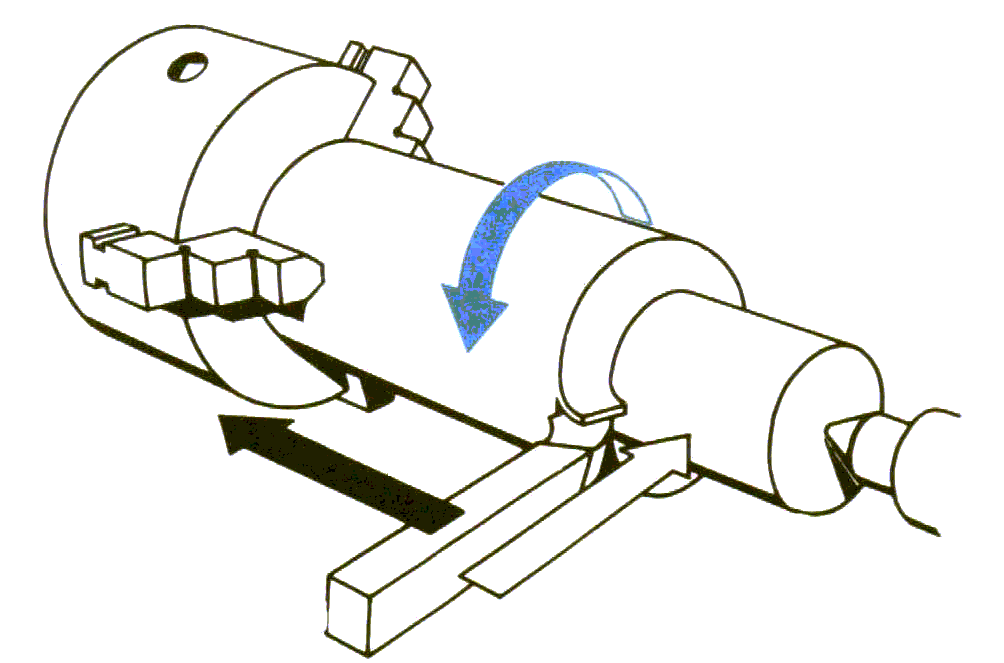
\includegraphics[width = 0.6\linewidth]{img/relat1/itornomove}
    \caption{Principais movimentos de um torno}
    \label{fig:torno}
\end{figure}

As principais operações de torneamento são:

\begin{figure}[H]
    \centering
    \begin{subfigure}[b]{0.3\textwidth}
        \centering
        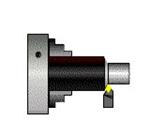
\includegraphics[width= 0.5\textwidth]{img/relat1/optornoExt}
        \caption{Torneameno Externo}
    \end{subfigure}
    ~
    \begin{subfigure}[b]{0.3\textwidth}
        \centering
        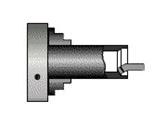
\includegraphics[width= 0.5\textwidth]{img/relat1/optornoInt}
        \caption{Torneameno Interno}
    \end{subfigure}
    ~
    \begin{subfigure}[b]{0.3\textwidth}
        \centering
        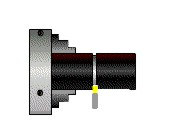
\includegraphics[width= 0.5\textwidth]{img/relat1/optornoSang}
        \caption{Sangramento}
    \end{subfigure}
    
    \begin{subfigure}[b]{0.3\textwidth}
        \centering
        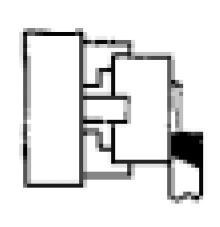
\includegraphics[width= 0.3\textwidth]{img/relat1/optornoFac}
        \caption{Faceamento}
    \end{subfigure}
    ~
    \begin{subfigure}[b]{0.3\textwidth}
        \centering
        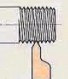
\includegraphics[width= 0.3\textwidth]{img/relat1/optornoRosq}
        \caption{Rosqueamento}
    \end{subfigure}
    ~
    \begin{subfigure}[t]{0.3\textwidth}
        \centering
        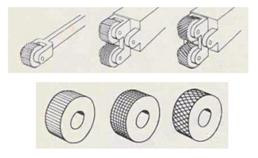
\includegraphics[width= 0.8\textwidth]{img/relat1/optornoReq}
        \caption{Recartilhamento}
    \end{subfigure}
    \caption{Operações de Torneamento}
\end{figure}

% Como Funciona
% Operações  
% Torno CNC

\subsubsection{Código G}
% Origem do Código G
% Funções Empregadas

\subsection{Linux CNC}\label{sec:linuxCNC}
% Descrição do Programa
O LinuxCNC, também chamado EMC2 (Enhanced Machine Controller, EMC), é um software controlador open-source disponibilizado de maneira gratúita com licença GNU/Linux que implementa a capacidade de Controle Numérico usando qualquer computador pessoal (PC) para controlar máquinas-ferramenta CNC de 3 a 9 eixos. O LinuxCNC usa Códigos G/M segundo a norma RS274NGC \cite{linuxcnc_2016}.

\subsection{Torno Didático}
Neste trabalho será utilizado como maquinário um torno didático desenvolvido por Magno Batista Correa para o laboratório GRACO da UnB.\cite{correia_2006}. O acionamento do rotor é feito por uma chave independente que ativa o motor DC ilustrado da figura \ref{fig:tornoCNC-pc}. O equipamento é controlado através do sistema \hyperref[sec:linuxCNC]{\textit{LinuxCNC}} por meio de instruções feitas em código G. Os comandos interpretados pelo LinuxCNC são convertidos em instruções para uma placa controladora acionando os dois motores de passo que controlam a posição da mesa no qual é posicionada a ferramenta de corte a ser utilizada permitindo apenas troca manual de ferramenta com máquina parada. 

\begin{figure}[H]
    \centering
    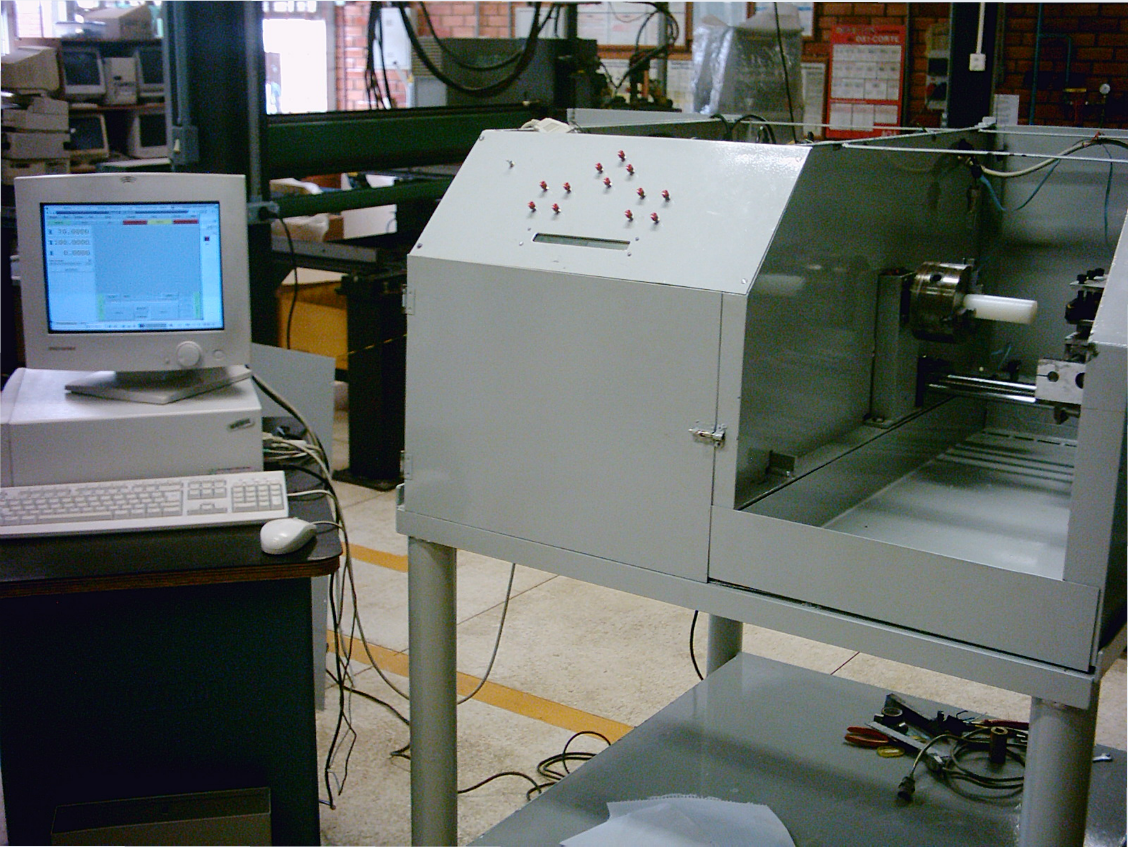
\includegraphics[width = 0.6\linewidth]{img/relat1/tornocnc}
    \caption{Torno CNC ligado ao computador (Extraído de \cite{correia_2006})}
    \label{fig:tornoCNC-pc}
\end{figure}

\begin{figure}[H]
    \centering
    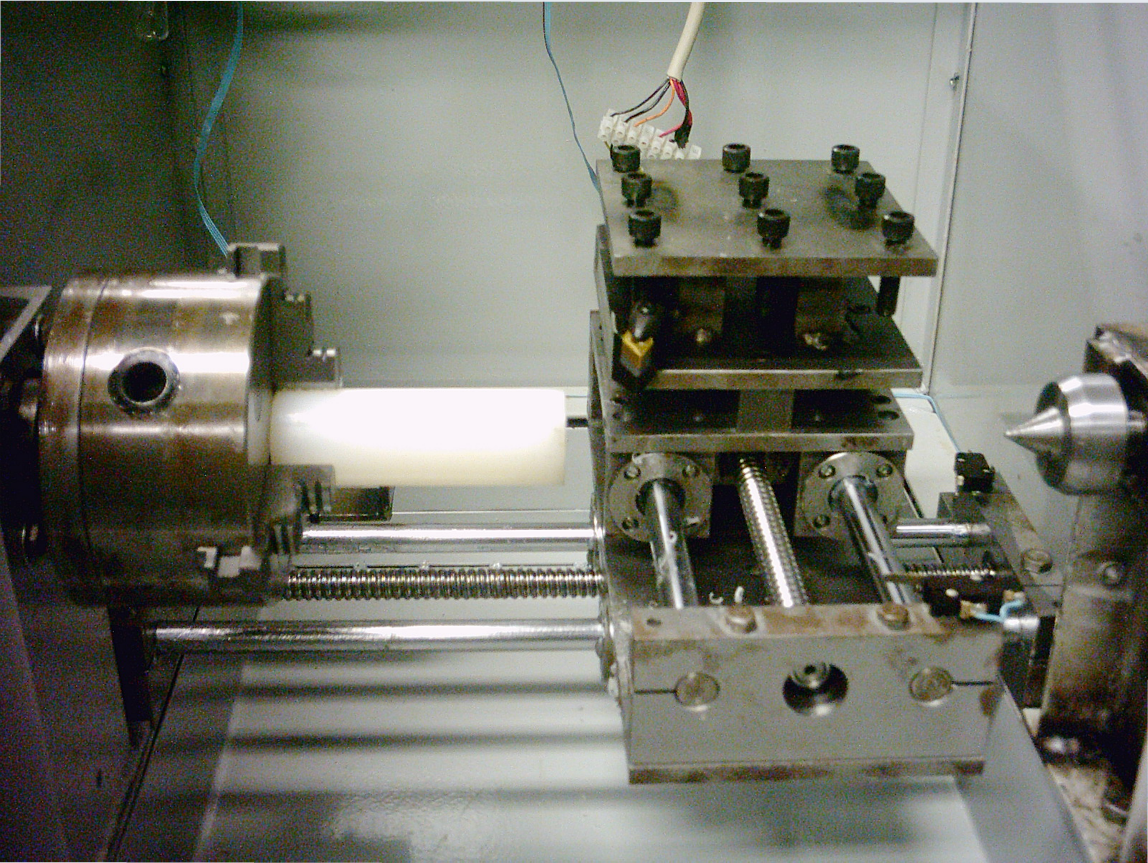
\includegraphics[width = 0.6\linewidth]{img/relat1/tornocnc2}
    \caption{Parte interna com os motores do Torno (Extraído de \cite{correia_2006})}
    \label{fig:tornoCNC-motores}
\end{figure}

\begin{figure}[H]
    \centering
    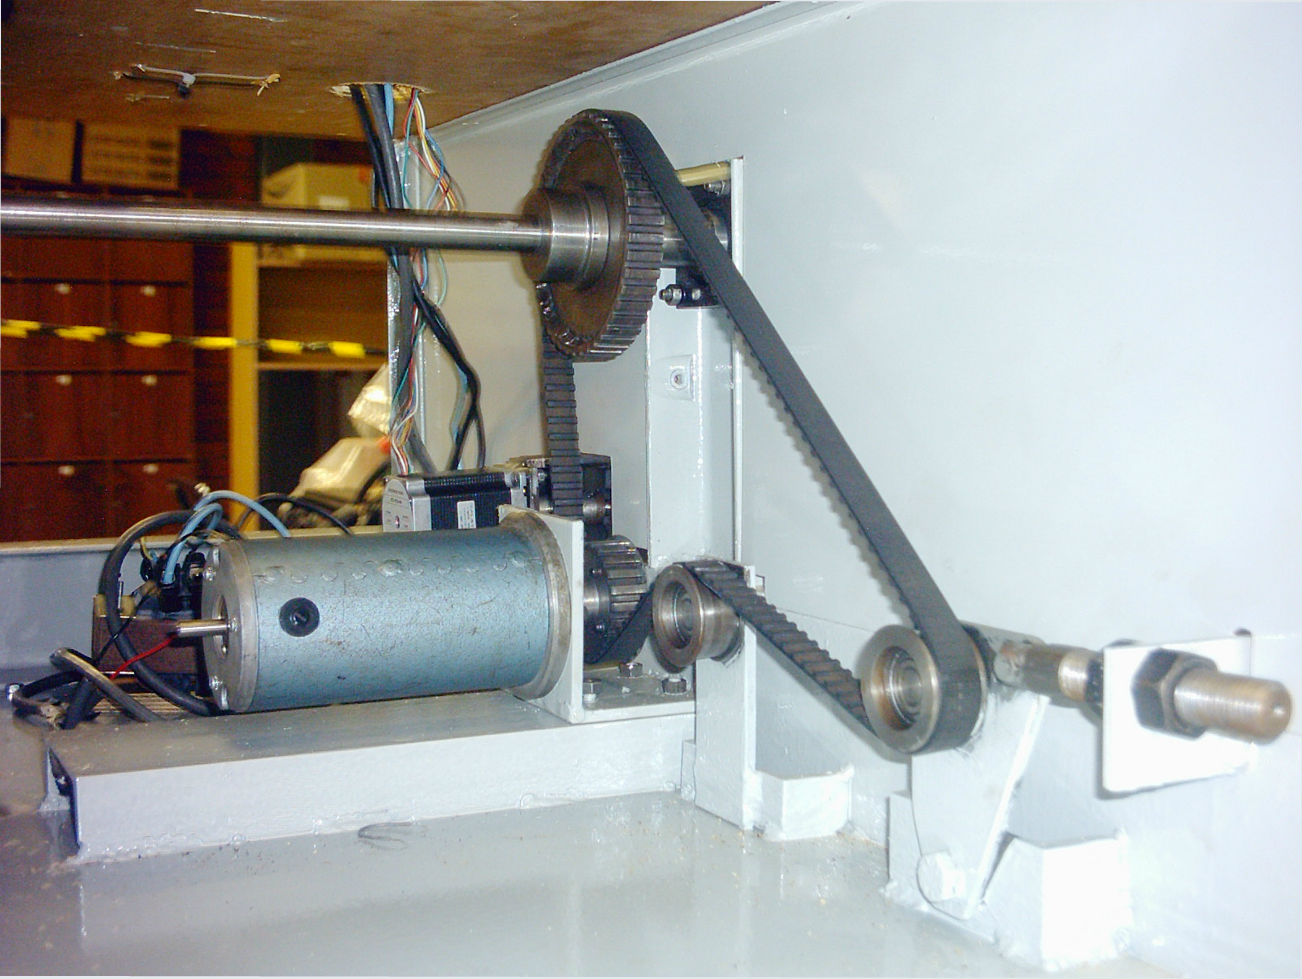
\includegraphics[width = 0.6\linewidth]{img/relat1/tornocnc3}
    \caption{Mesa de fixação da ferramenta e castanha com uma vela fixada (Extraído de \cite{correia_2006})}
    \label{fig:tornoCNC-mesa}
\end{figure}

%\subsection{Estudo de Capabilidade}
% Fontes de Erro de Medida
% Recomendações para evitar erros

\section{Procedimentos}
 Será usinado uma vela maciça de $150\ mm$ feita de parafina colorida. Tal material foi escolhido em razão de permitir fácil usinagem com poucos esforços com pouco esforços para a ferramenta de corte permitindo a avaliação de diferentes geometrias sem o risco de quebra da ferramenta. 

\subsection{Projeto da Peça}
Primeiramente a peça foi desenhada em papel milimetrado. Para o desenho foram exploradas 2 tipos de operações: torneamento externo para desbaste, corte reto com angulação em relação ao eixo de peça e corte com interpolação circular e sangramento. Desta forma poderiam ser feito a avaliação da precisão do torno ao longo do eixo $X$ e $Z$. Será utilizado apenas uma ferramenta de sangramento para a execução de todas as operações. Tal somente é possível devido a usinagem da parafina exigir pouco esforços da ferramenta para o emprego de outros materiais a troca de ferramenta entre cada etapa poderá ser necessária visando adequar a melhor para o tipo de operação exigida.

\subsection{Simulação}
\subsubsection{CNC Web Simulator}
O desenho inicial da vela foi avaliado utilizando o sistema CNC Web Simulator desenvolvido pelo Felipe Caixeta.\cite{filipecaixeta_2016} A escolha deste  simulador foi por este permitir uma rápida análise do efeito de cada instrução no desenho final da peça. Inicialmente foi determinado apenas o desenho final da peça e após validação do formato desejado foram adicionadas as etapas de desbaste para cada região da peça conforme ilustrado na figura \ref{fig:vela-simCNCWebSimulator}.

\begin{figure}[H]
    \centering
    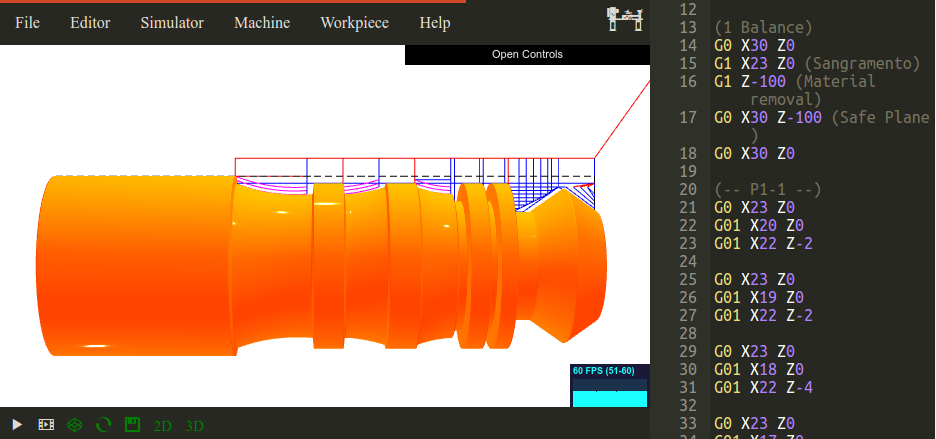
\includegraphics[width = 0.6\linewidth]{img/relat1/sim-webcnc}
    \caption{Simulação no Sistema Web CNC  Simulator}
    \label{fig:vela-simCNCWebSimulator}
\end{figure}

\subsubsection{LinuxCNC}
Uma vez feita terminado a avaliação das etapas de desbaste procedeu-se com a simulação do caminho de ferramenta dentro do sistema LinuxCNC. Este passo foi fundamental para a avaliação do caminho de ferramenta tomado ao longo do processo de usinagem uma vez que o mesmo sistema será utilizado para o controle do Torno CNC Educacional. O zeramento da ferramenta é feito tomando-se a posição inicial no programa e a simulação ocorre indo da direita para esquerda em conformidade com o que ocorrerá na usinagem.

\begin{figure}[H]
    \centering
    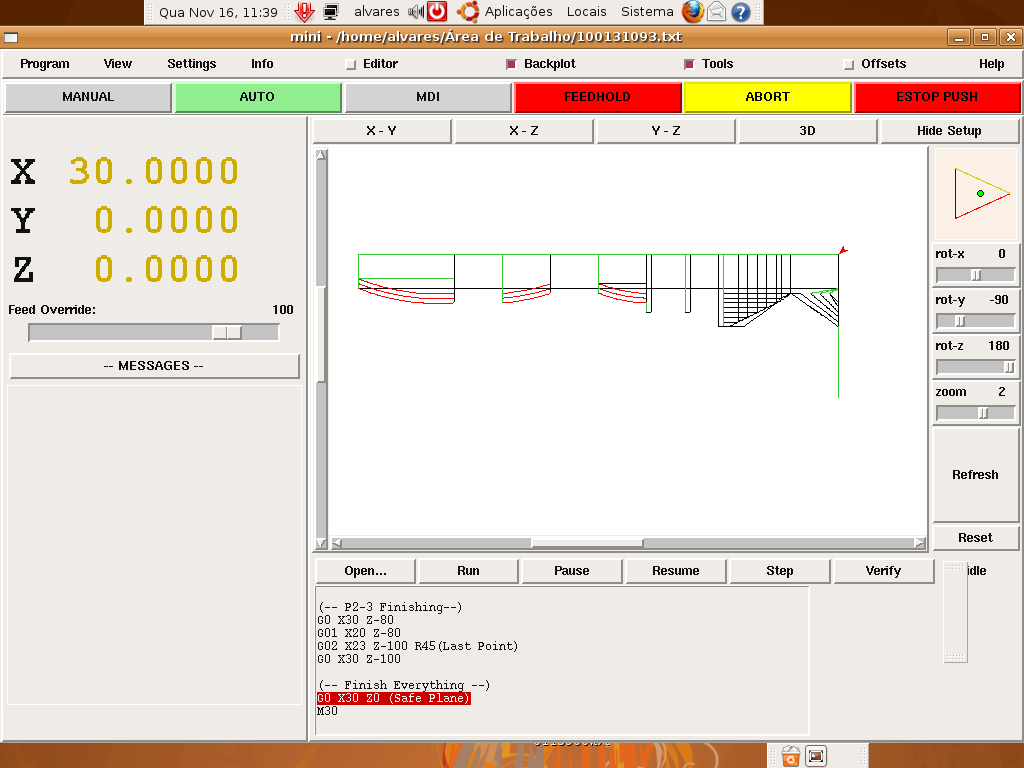
\includegraphics[width = 0.6\linewidth]{img/relat1/simLinuxCNC}
    \caption{Simulação no Linux CNC}
    \label{fig:vela-simLinuxCNC}
\end{figure}

\subsection{Torneamento}
Para a etapa de torneamento foram modificadas todas movimentações em $G0$ para $G01$ no código G pois o torno conta com apenas uma velocidade e em seguida procedeu-se da seguinte maneira:
\begin{enumerate}
    \item Fixação da Vela na Castanha do torno
    \item Upload do código na máquina de controle através de um Disquete 3/4"
    \item Zeramento da posição da mesa através do posicionamento no eixo $Z$ da ponta da ferramenta na extremidade da vela com auxilíio do programa Linux CNC.
    \item Acionamento do rotor através da chave de Liga/Desliga
    \item Início da execução programa da Peça atráves do LinuxCNC
    \item Remoção do cavaco com auxílio de arame com a usinagem em andamento para evitar travamento da mesa.
    \item Desligamento do rotor através da chave de Liga/Desliga ao fim da usinagem.
    \item Remoção da vela da castanha.
\end{enumerate}

Todas as etapas foram feitas utilizando-se a mesma ferramenta de corte sem a remoção ou o reposicionamento da peça no torno. O resultado final encontra-se na figura {} aonde mostra a vela acabada ainda dentro do torno.

\begin{figure}[H]
    \centering
    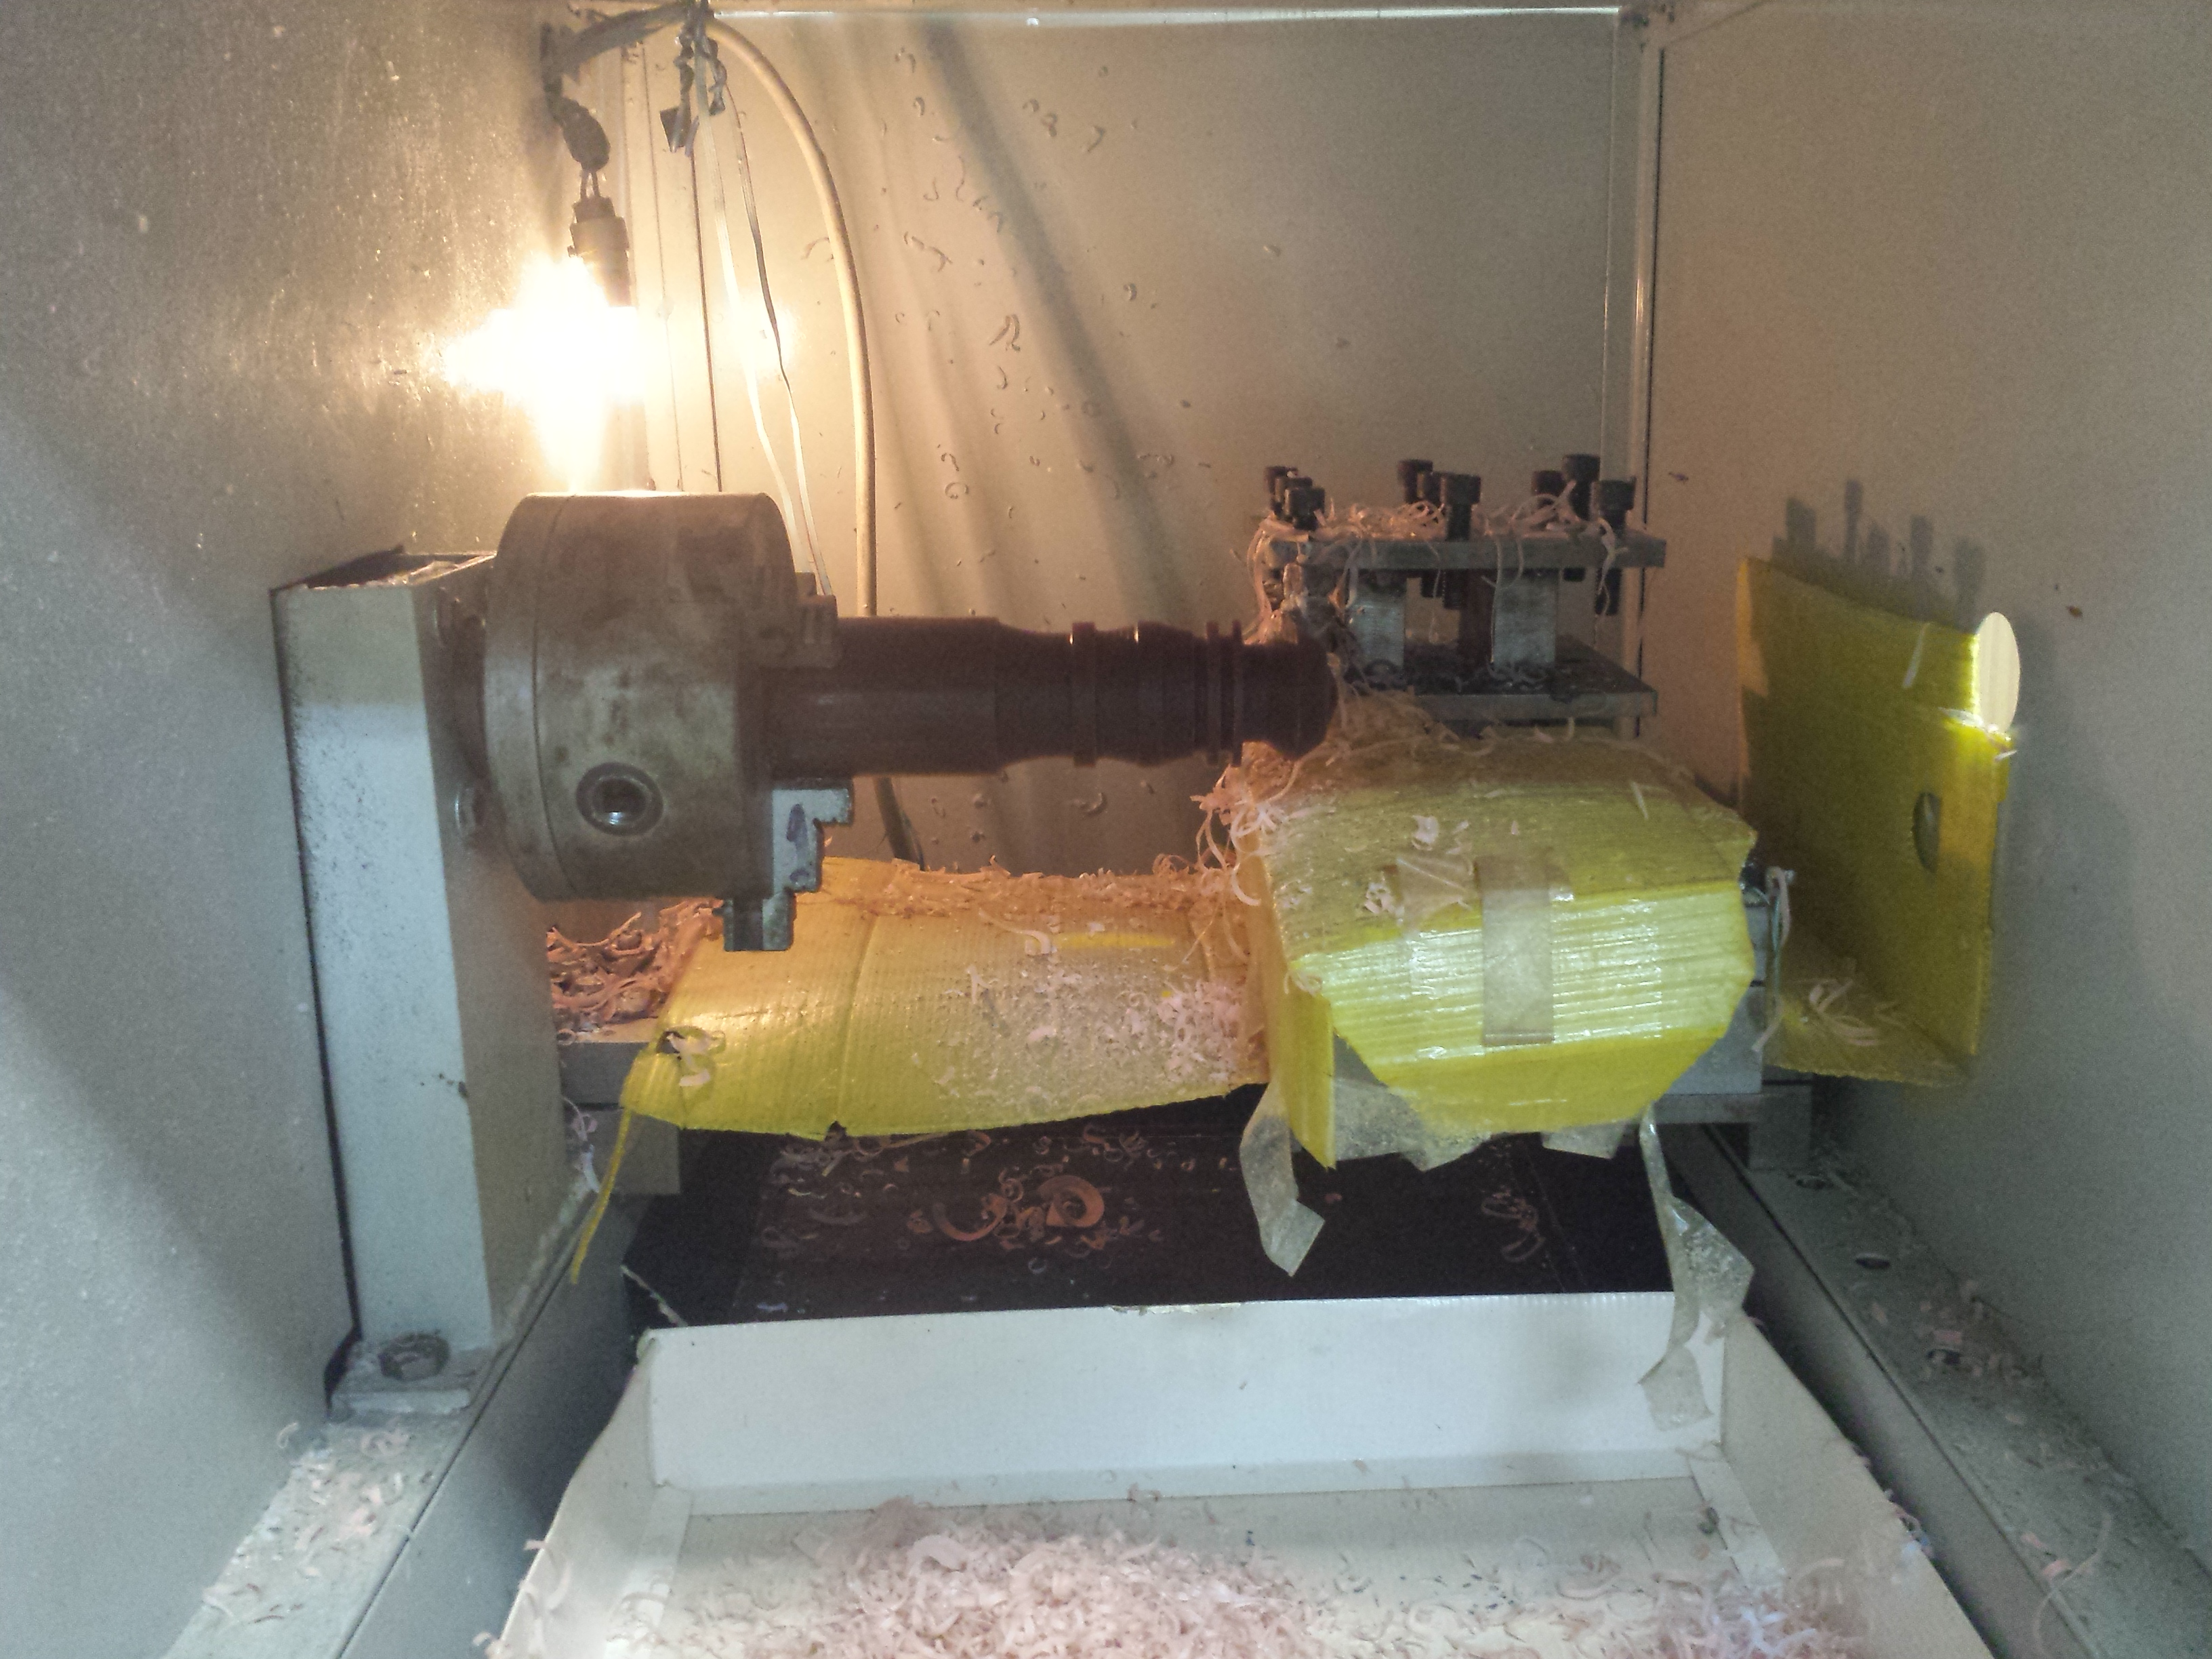
\includegraphics[width = 0.6\textwidth]{./img/relat1/vela-torno}
    \caption{Vela acabada dentro do Torno}
    \label{fig:vela_tornoCNC}
\end{figure}

\begin{figure}[H]
    \centering
    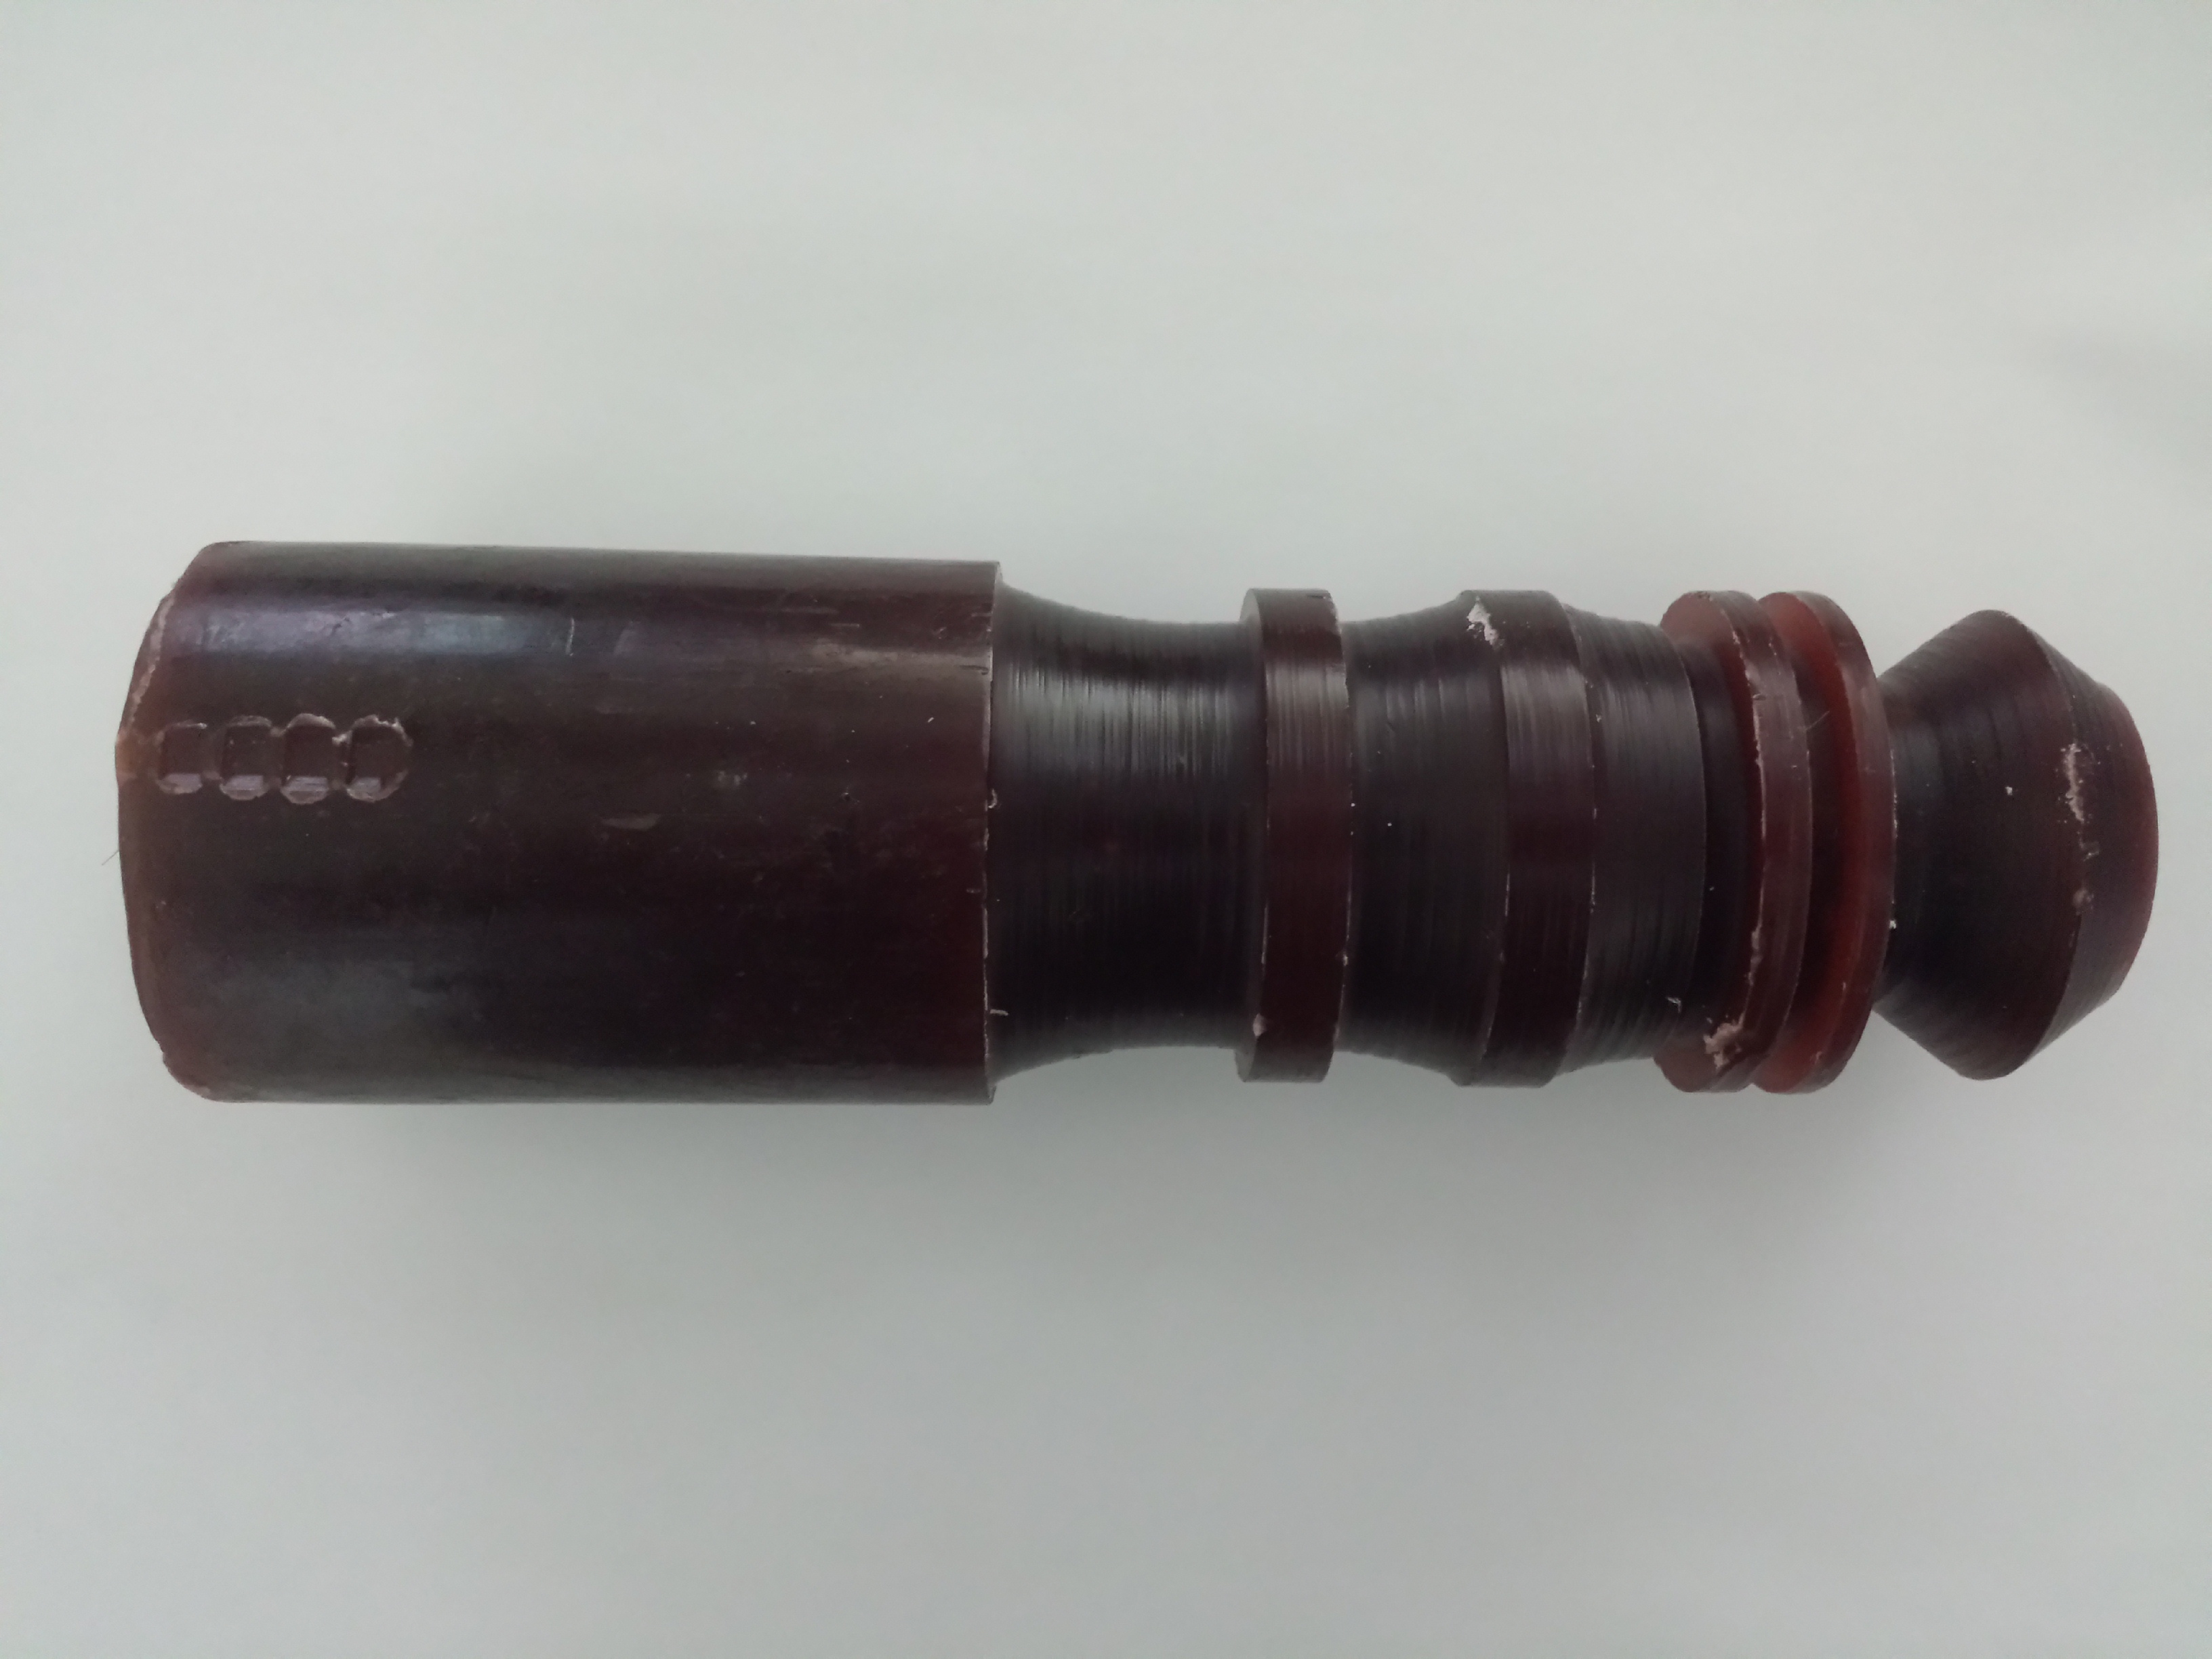
\includegraphics[width = 0.6\textwidth]{./img/relat1/vela-detalhe}
    \caption{Vela acabada}
    \label{fig:vela_final}
\end{figure}


\subsection{Métrica da Vela}
Para avaliar a qualidade de cada operação foram feitas diversas medidas na vela em diferentes posições ao longo de seu comprimento e em comparadas com os valores iniciais de projeto.

\begin{figure}[H]
    \centering
    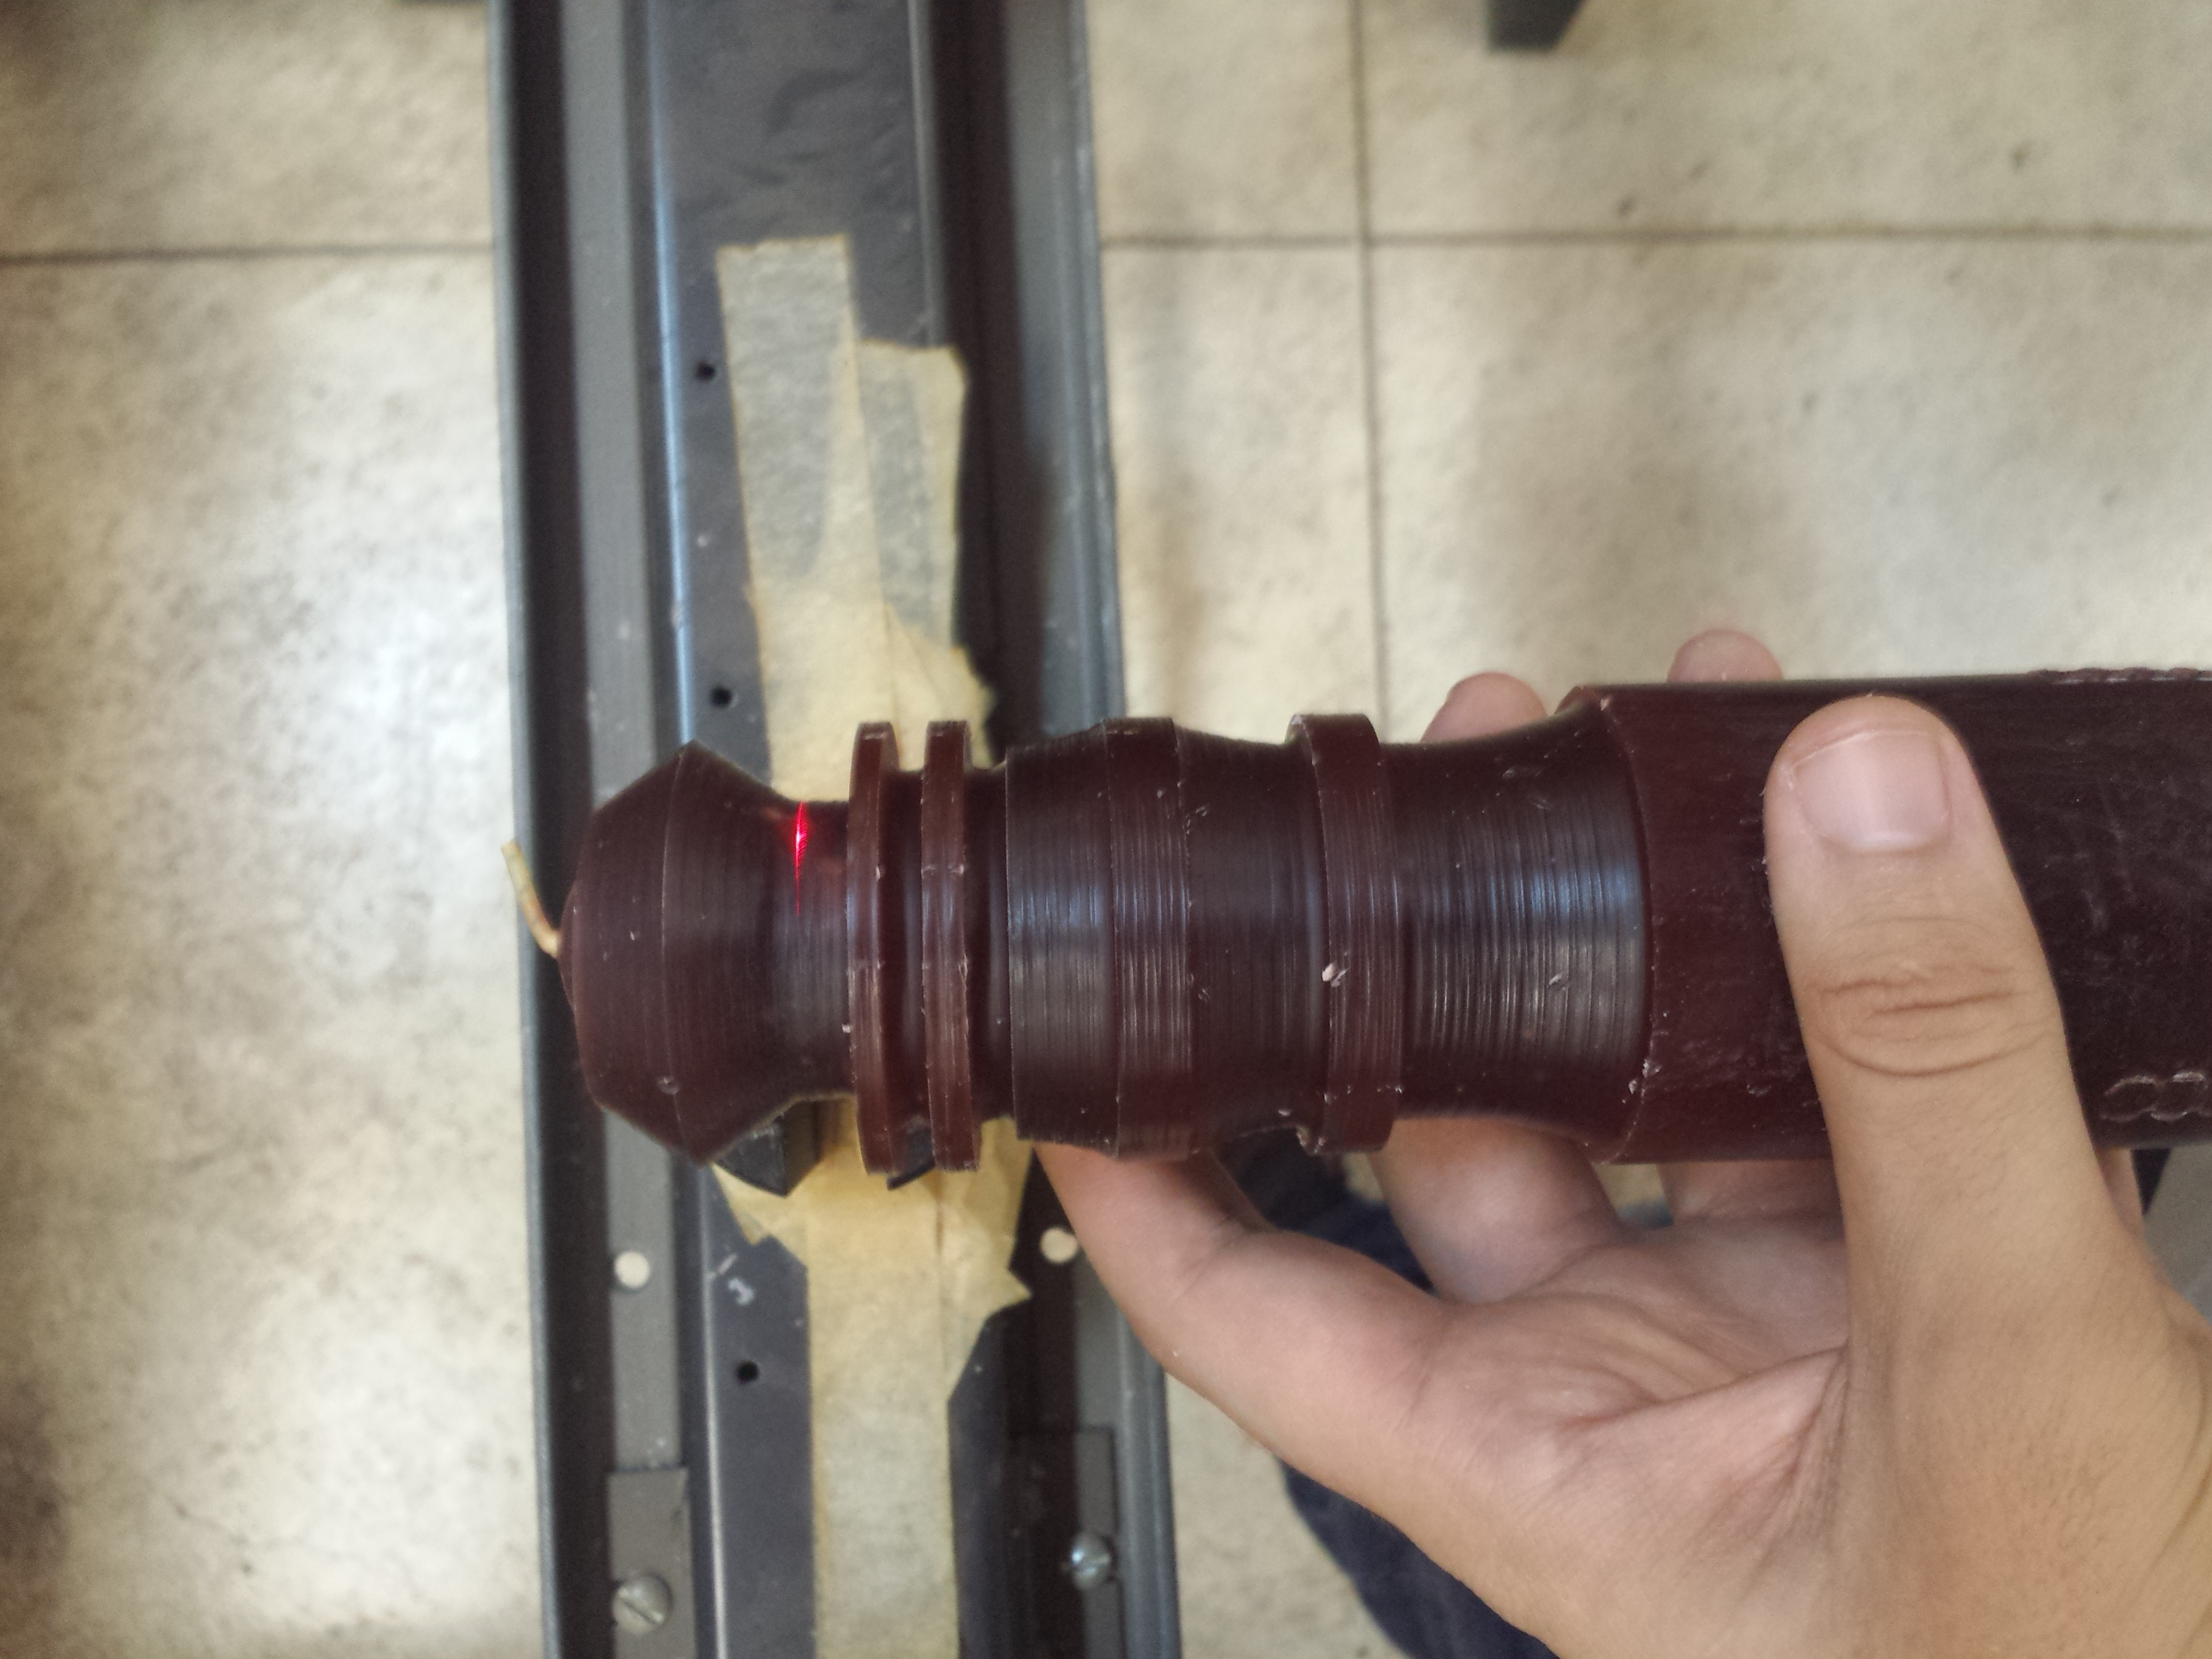
\includegraphics[width = 0.6\textwidth]{./img/relat1/vela-medidas}
    \caption{Medições na vela}
    \label{fig:vela_medidas}
\end{figure}

\begin{table}[H]
    \centering
    \begin{tabular}{cccc}
    \hline
        & & \multicolumn{2}{c}{Peça}\\
        Posição & Projeto & Média & Variância\\
    \hline
         & & &\\
         & & &\\
    \hline
    \end{tabular}
    \caption{Medidas da Peça}
    \label{tab:my_label}
\end{table}

\section{Discussão}
 Em razão da diâmetro da ferramenta é percebido uma região reta no inicio das regiões feitas utilizando interpolação circular. Foi percebido também a presença de uma leve curvatura na cavidade interna das regiões aonde foi feito o sangramento junto a um leve faceamento. Tal pode ser explicado devido ao desgaste na ponta da ferramenta que confere menos precisão ao corte.

\section{Conclusão}
% Avaliação dos resultados
Peça usinada foi concluída com sucesso, permitindo a confecção de todas as formas originais de projeto. A usinagem apresentou um leve desvio nas medidas de raio conferindo

% Prototipagem Rápida



% Referências ----------------------------------------------------------------------------------------------------------------------

\bibliographystyle{plain}
\bibliography{reference}


% Magno Correa
% http://buscatextual.cnpq.br/buscatextual/visualizacv.do?id=K4734325E3
% https://prezi.com/user/j4f46ctrnc3o/

% LinuxCNC
% https://en.wikipedia.org/wiki/LinuxCNC
% http://linuxcnc.org/docs/2.7/html/getting-started/about-linuxcnc.html

% ----------------------------------------------------------------------------------------------------------------------------------
\end{document}
